\documentclass[twoside=false,DIV=14]{scrartcl}

\usepackage{arev} % order matters, putting this above allows FiraSans to override it for body text
\usepackage[sfdefault]{FiraSans}
\usepackage{inconsolata}
%\usepackage[fira]{fontsetup}
\usepackage{scrlayer-scrpage}
\renewcommand{\titlepagestyle}{scrheadings}
\usepackage{graphicx}
\usepackage{blindtext}
\usepackage{wrapfig}
\usepackage{tabularx}
\usepackage{hyperref}
\usepackage{listings}
\usepackage{tikz}
\usepackage{amsmath}
\usepackage[many]{tcolorbox}

\usepackage{xcolor,sectsty}
\definecolor{blackish}{RGB}{56,58,54}
\definecolor{redish}{RGB}{109,41,49}
\definecolor{red}{RGB}{152,41,50}
\definecolor{orangeish}{RGB}{188,71,0}
\definecolor{blueish}{RGB}{25,33,139}
\subsubsectionfont{\color{blackish}}
\subsectionfont{\color{blackish}}
\sectionfont{\color{blackish}}

\lohead{\color{red} COMP3000 Programming Languages}
\rohead{
\includegraphics[width=0.5cm]{../logo.jpg}}

\setkomafont{author}{\sffamily \small}
\setkomafont{date}{\sffamily \small}

\DeclareOldFontCommand{\bf}{\normalfont\bfseries}{\mathbf}
\DeclareOldFontCommand{\tt}{\normalfont\ttfamily}{\texttt}

\lstset{basicstyle=\ttfamily}


\date{}
\newtcolorbox{aside}[1][]{
  title=Aside,
  width=0.3\textwidth,
  fonttitle=\bfseries,
  breakable,
  fonttitle=\bfseries\color{black},
  colframe=blueish!80,
  colback=blueish!2
  #1}

\newtcolorbox{note}[1][]{
  title=Note,
  width=\textwidth,
  fonttitle=\bfseries,
  breakable,
  fonttitle=\bfseries\color{black},
  colframe=orangeish!80,
  colback=orangeish!2
  #1}

\newtcolorbox{hint}[1][]{
    title=Hint,
    width=\textwidth,
    fonttitle=\bfseries,
    breakable,
    fonttitle=\bfseries\color{white},
    colframe=blueish!80,
    colback=blueish!2
    #1}

\newtcolorbox{todo}[1][]{
  title=!! TODO !!,
  width=\textwidth,
  fonttitle=\bfseries,
  breakable,
  fonttitle=\bfseries\color{white},
  colframe=red!80,
  colback=red!2
  #1}
  
\providecommand{\tightlist}{%
  \setlength{\itemsep}{0pt}\setlength{\parskip}{0pt}}

\usepackage{amssymb}

\usepackage{listings}
\lstset{basicstyle=\ttfamily}

\renewcommand{\theenumi}{\alph{enumi})}

\title{\color{redish} \vspace{-2em}COMP2010: Relevant Past Exam Questions}

\begin{document}
{\color{blackish}\maketitle}\vspace{-2em}
Exam questions from the first half of the unit generally fit into one of five question styles:
\begin{enumerate}
\item Recursive Data, Recursion, and Recursion/Iteration Isomorphism
\item Divide and Conquer, Invariants, and Complexity
\item Dynamic Programming.
\item Advanced Sort, Invariants, and Complexity
\item Binary Search Trees and Binary Trees
\end{enumerate}
We have collected past exam questions in each style for easy study.  We have even made adjustments to the questions to account for differences in 2025.

\newpage\setcounter{section}{0}
\part*{Recursive Data, Recursion, and Recursion/Iteration Isomorphism}

\section{2022 Final Exam Question 1}
\begin{note}
In 2022, doubly linked lists and queues were covered in lectures. I think you are capable of doing this question since there are no new concepts, its just another recursive data type.  I have adjusted this question a little to make it easier for 2024 students.
\end{note}
Consider the following definition of a node for a doubly-linked list together with a constructor. Refer to this in the parts of this question below.

\begin{lstlisting}
public class DLL {
  char key;
  DLL next;
  DLL prev;
  
  DLL(char el) {
    key= el;
    next= null;
    prev= null;
  }

  DLL(char el, DLL n, DLL p){
    key = el;
    next  = n;
    prev = p;
  }
}       
\end{lstlisting}

\begin{enumerate}
\item (3 marks) Consider the following code snippet where tail (initially) is a reference to the last node in a doubly-linked list which has already been initialised like this.
\begin{lstlisting}
DLL list = new DLL('a');
DLL tail = list;
list = new DLL('b', list, null);
list = new DLL('c',list, null);
\end{lstlisting}
Complete the lines indicated at \verb+????+ so that the completed code adds the new node containing \verb+'Z'+ to the end of the linked list, and updates tail so that it points to the just added node.
\begin{lstlisting}
    DLL y = new DLL('Z');
    ????
    ???? 
\end{lstlisting} 

\begin{figure}
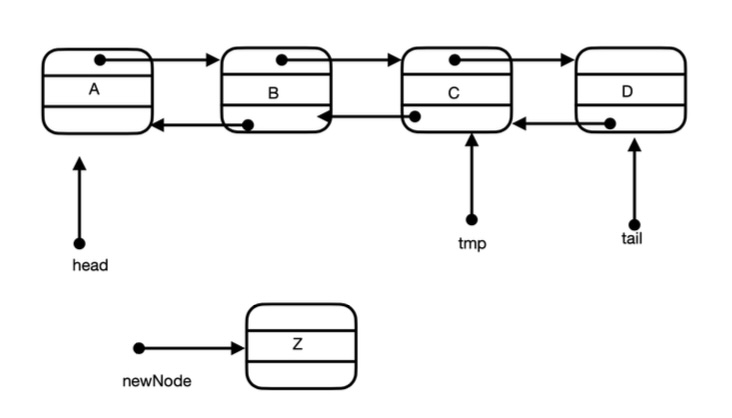
\includegraphics[width=0.8\textwidth]{./2022_q1.jpg}
\label{fig:dll}
\caption{Use this to answer parts (b–g)}
\end{figure}
Use the diagram in Figure \ref{fig:dll} in parts (b–g) below. Note that head is a reference to the first node of the depicted list, tail is a reference to the last node, and tmp is a reference to the node containing C. Finally \verb+newNode+ is a node that has been declared and initialised. Note that in Figure 1, the upper arrow of any node x corresponds to x.next and the lower arrow corresponds to y.prev of any node y. In your diagrams below you must indicate which nodes head, tail, tmp and newNode refer to.

\item (2 marks) Assume that the list is initially as in Figure 1. Redraw the list after executing the following code snippet.
\begin{lstlisting}
        newNode= tmp.next;
\end{lstlisting}
\item (2 marks) Assume that the list is initially as in Figure 1. Redraw the list after executing the following code snippet.
\begin{lstlisting}
        newNode.next= tmp.prev;
        newNode.prev= tmp;
\end{lstlisting}
\item (2 marks) Assume that the list is initially as in Figure 1. Redraw the list after executing the following code snippet.
\begin{lstlisting}
        tail.next= head;
        head.prev= tail;
\end{lstlisting}
\item Assume that the list is initially as in Figure 1. Redraw the list after executing the following code snippet.
\begin{lstlisting}
    newNode.prev= tmp.prev;
        tmp.prev= newNode;
        newNode.next= tmp;
        newNode.prev.next= newNode;
    \end{lstlisting}
Assume that the list is initially as in Figure 1. Parts (f–h) concern the following program.
\begin{lstlisting}
   while(head!= tail) {
    System.out.println(tail.key);
    tail= tail.prev;
   } // LINE 4
   while (head.next!=null) {
    System.out.println(head.key);
    head= head.text;
   } // LINE 8
\end{lstlisting}
\item (2 marks) Redraw the list after completely executing the first while loop (i.e. up until LINE 4). You must indicate which nodes head, tail, tmp and newNode point to.
\item (2 marks) Redraw the list after completely executing the whole program (i.e. up until up until LINE 8). You must indicate which nodes head, tail, tmp and newNode point to.(Only draw the state of the final list.)
\item (4 marks) What does the whole program above output? (Assume that the whole program executes up until LINE 8.)

Parts (i–m) concern the following partially-implemented class for a Queue (which uses DLL). Recall that a Queue is implemented by a list-like data structure; items are added to the back of the Queue, and removed from the front of the Queue.
{\small\begin{lstlisting}
class Queue {
  DLL first= null; // Records the element at the front of the queue;
  DLL last= null; // Records the element at the back of the queue

  Queue () { // Default constructor

  void qPush(char x) { ... } // Creates a DNode containing
                             // x and adds it to the back of the queue

  char qPop() {...} // Removes the first node (if it exists) of the
                    // queue and returns the value (of the removed node);
                    // returns null if the queue is empty.
}
\end{lstlisting}}
\item Provide an implementation for \verb+qPush(char x)+
\item Write down the complexity for your implementation.
\item (3 marks) Provide an implementation for \verb+qPop()+
\item (1 mark) Write down the complexity for your implementation.
\item (3 marks) Now consider a priority queue where the priority is defined by alphabetical order on characters of key. Explain whether and how the implementation of Queue needs to be changed and how your suggested changes (if any) affect the implementations of \verb+qPop+ and/or \verb+qPush+. If the complexity of \verb+qPop+ or \verb+qPush+ changes, state in what way. Write no more than FIVE lines.
\end{enumerate}

 

\newpage\setcounter{section}{0}
\part*{Divide and Conquer, Invariants, and Complexity}

\section{2024 Mid Semester Exam Question 3}
Which statements are true of the term "Divide and Conquer"?  Choose all that apply.  Note that incorrect choices accrue negative marks.
\begin{enumerate}
\item[$\square$] It is a technique to compute the Fibonacci numbers.
\item[$\square$] It is a design strategy that can be used effectively to implement some sorting algorithms.
\item[$\square$] Whenever it is applied, it always saves resources.
\item[$\square$] It uses the results of sub-problems to compute a result for the whole problem.
\item[$\square$] It is a design strategy to implement recursion.
\end{enumerate}

 

\section{2022 Final Exam Question 2}
This question is about divide and conquer algorithms studied in lectures.

\begin{enumerate}
\item (6 marks) Explain the term divide and conquer. Give and example to illustrate your
answer. Write no more than SIX lines.


Consider the following program which has an incomplete precondition (???) and a com- plete postcondition. Assume that the array A containing N integers, and the given integer key, have both already been initialised.
{\small\begin{lstlisting}
// Precondition: ???
// Postcondition: set index i so that 0 < i < N AND  A[i-1]< key <= A[i]
//                set index i to N if no such value for i can be found
first= 0; last= N;
while(first!=last) {
     mid= (first+last)/2;  // LINE 3
     if (A[mid] < key) then first= mid+1;
     else last= mid;
} // LINE 6
i= ????? // LINE 7
\end{lstlisting}}
Note that at LINE 3 the division is integer division, which means that if \verb+first + last+ is odd then \verb+(first+last)/2+ is the floor of the result of ordinary division. For example if \verb+first + last = 7+ then \verb+(first+last)/2 == 3+.

Also, $0 < i < N$ means that i must be strictly bigger than 0 and strictly smaller than N, and $A[i-1]< key <= A[i]$ means that $A[i-1]$ must be strictly less that key and that $A[i]$ must be at least key.

\item (3 marks) If \verb+A=[2, 5, 1, 3, 8, 6]+ and \verb+key=5+, what will the value of index last be at LINE 6 (after the loop has terminated)?
\item (3 marks) If \verb+A= [1, 2, 2, 5, 6, 8]+ and \verb+key=5+, what will the value of index last be at LINE 6 (after the loop has terminated)?
\item (3 marks) If \verb+A= [1, 2, 2, 5, 6, 8]+ and \verb+key=2+, what will the value of index last be at LINE 6 (after the loop has terminated)?
\item (3 marks) If \verb+A= [1, 2, 2, 5, 6, 8]+ and \verb+key=3+, what will the value of index last be at LINE 6 (after the loop has terminated)?
\item (2 marks) Using your answers above, or otherwise, write a precondition for the program, to ensure that the postcondition can always be satisfied for the initial values key and A satisfying your stated precondition. Your precondition should only mention \verb+key+ and \verb+A+.
\item (2 marks) For your precondition above, complete the assignment at LINE 7 so that the program satisfies the given postcondition. (Hint: You might need to use a conditional.)
\item (2 marks) What is the worst-case complexity of the program in terms of the length of the array A?
Parts (i) and (j) concern using the program above to find integer cubed roots. 

Given a number $k>0$,its integer cubed root $r$ is the value such that $(r-1)^3 < k < r^3$.
\item (3 marks ) Assume you are given an array
\begin{lstlisting}
   cubes = [0, 1, 8, 27, 64, 125, ...  , 1000]
\end{lstlisting}
of the first ten cubed numbers, so that \verb+cubes[i] = i*i*i+ for 0  i  10. Show how you would use the program above to compute the integer cube root for any number $k$ such that $0 < k < 1000$.
\item (3 marks ) Using your answer above or otherwise, write an efficient program using a divide and conquer strategy that delivers the integer cubed root for any input number. You must not use an array in your implementation.
\begin{lstlisting}
   int cubedRoot(int k)
   // Precondition: k > 0
   // Postcondition: returns the integer cubed root of k.
\end{lstlisting}
\end{enumerate}

 

\section{2024 Mid-Semester Exam Question 2}
Consider the following program. What is the correct assignment to temp at ???? which will ensure that the correct result (i.e. $x^{exp}$) is returned?
\begin{lstlisting}
int power (int exp, int x) {
 if (exp==0) return 1;
 else {
   int temp= ????
   if (exp%2 == 0) return temp;
   else return temp*x;
 }
}  
\end{lstlisting}
 

% TODO: this question set (which is in iLearn) seems completely buesed.
% \section{2024 Mid-Semester Exam Question 3}
% Consider the following algorithm based on question (2).  If \verb+exp+ is initially 9 how many recursive calls will be made?
% \begin{lstlisting}
% int power (int exp, int x) {
%     if (exp==0) return 1;
%     if (exp==1) return x;
%     else {
%         int temp= ????
%         if (exp%2 == 0) return temp;
%         else return temp*x;
%     }
% }
% \end{lstlisting}

%  

\newpage\setcounter{section}{0}
\part*{Dynamic Programming}

\section{2024 Mid-Semester Exam Question 1}
Which sentences best describe the term Dynamic Programming?  Select only statements that apply -- incorrect selections receive negative marks.
\begin{enumerate}
\item[$\square$] It is a technique that stores partial results to be used for subsequent calculations.
\item[$\square$] It is only effective for some recursive solutions.
\item[$\square$] It is a design strategy to implement recursion.
\item[$\square$] It always saves resources when it is used.
\item[$\square$] It is a technique to compute tables.
\end{enumerate}

\newpage

\section{2025 Final Exam}
We are playing a game.  The rules of the game are:
\begin{itemize}
    \item Players take turns making moves.
    \item The \emph{score} of each move is calculated as $score(move) = score(move-1) + score(move -2)*score(move-3)$ where the first three scores are $score(1) = 1$, $score(2) = -1$, $score(3) = 2$.
    \item A player who gets a score of $0$ on a move which is a \emph{prime number} will win the game.
\end{itemize}

\begin{enumerate}
\item (5 marks) Calculate the score for the number 1-10.  Which is the winning move?
\item (5 marks) Write an $O(n^3)$ recursive algorithm which computes the score for any given move.
\item (5 marks) Write an $O(n))$ dynamic algorithm which computes the score for any given move.
\end{enumerate}

 

\newpage\setcounter{section}{0}
\part*{Advanced Sort, Invariants, and Complexity}

\section{2023 Final Exam Question 2}
\begin{note}
A different version of quicksort was used in 2023.  I have updated this question to use the 2025 version thus the text below is slightly different to the 2023 text.
\end{note}
Consider the following code for Quicksort. Refer to this in the parts of this question below.
{\small\begin{lstlisting}
void swap(char[] a , int i, int j) {
    char temp= a[i];
    a[i]= a[j];
    a[j]= temp;
}

int partition(char[] a, int first, int last){
    char pivot = a[first];
    int L = first;
    int R = first+1;
    while(R <= last){
        // INVARIANT: ???? pre-condition: ???? post-condition: ????
        if (a[R] < pivot){
            L++;
            swap(a,L,R);
            R++;
        } else {
            R++;
        }
    }
    swap(a,first,L);
    return L;
}

void sort(char[] a, int first, int last) {
    if (first < last) {
        int pivot = partition(a, first, last); // update pivotIndex
        sort(a, first, pivot-1);
        sort(a, pivot +1, last);
    }
}
\end{lstlisting}}
\begin{enumerate}
\item (8 marks) Give the Invariant, pre-condition and post-condition on the order of the array in the main loop (at ????).
\item (5 marks) Explain (in no more than 5 lines) how Quicksort is using Divide and Conquer strategy.

\item (5 marks) Suppose you are given an array A of n sorted numbers that has been circularly shifted k positions to the right. For example,
\begin{verbatim}
{35, 42, 5, 15, 27, 29}
\end{verbatim}
is a sorted array that has been circularly shifted k = 2 positions, while
\begin{verbatim}
{27, 29, 35, 42, 5, 15}
\end{verbatim}
has been shifted k = 4 positions.
\begin{enumerate}
\item What is the complexity (in O() notation) of the above Quicksort execution if k = 0?
\item What is the complexity (in O() notation) of the above Quicksort execution if k = n - 1?
\end{enumerate}
\item (8 marks) Assume that the above Quicksort is executed with sort(A, 0, 5) where A is:
\begin{verbatim}
A = {27, 38, 12, 39, 28, 16}
\end{verbatim}
\begin{enumerate}
\item How many times will the item 27 be moved during the first call to \verb+partition(A, 0, 5)+?
\item How many times will the item 38 be moved during the first call to \verb+partition(A, 0, 5)+?
\item In O() notation, what is the maximum number of moves of an array item during the
first call to \verb+partition(A, 0, n-1)+?
\item How many times will the item 27 be moved in total during the execution of \verb+sort(A, 0, 5)+?
\end{enumerate}
\end{enumerate}
 

\section{2024 Final Exam Question 2}
\begin{note}
The merge sort code in 2025 differs from 2024. This question has been changed here to match the 2024 version.
\end{note}
Consider the following code for Merge in Mergesort. Refer to this in the parts of this question below.
{\small\begin{lstlisting}
public static char[] sort(char[] unsorted){
    if (unsorted.length == 1)
        return unsorted;
    int    mid   = unsorted.length/2;
    char[] left  = sort(Arrays.copyOfRange(unsorted, 0, XXXX));
    char[] right = sort(Arrays.copyOfRange(unsorted, XXXX, YYYY));
    return merge(left, right);
}

// PRE: the array portions A[a..mid-1] and A[mid..b] are sorted
// POST: The array portion A[a..b] are sorted
    public static char[] merge(char[] left, char[] right){
    // INVARIANT for all the loops:
    // tA[0.. (i-a) + (j-mid) -1] is the sorted merge of A[a..i-1] and A[mid..j-1]
    char[] ret = new char[left.length + right.length];
    int i = 0;
    int j = 0;
    while (i < left.length && j < right.length){
        if(left[i] < right[j]){
            ret[i+j] = left[i];
            i++;
        } else {
            ret[i+j] = right[j];
            j++;                
        }
    }
    // flush the left
    while (i < left.length){
        ret[i+j] = left[i];
        i++;
    }

    // flush the right
    while (j < right.length){
        ret[i+j] = right[j];
        j++;
    }
    return ret;
}
\end{lstlisting}}
\begin{enumerate}
\item (6 marks) Complete the lines indicated at\verb+XXXX+ and \verb+YYYY+ so that the completed code sorts the array \verb+unsorted+. Just write “XXXX= ...” and “YYYY= ...” respectively.
\item (6 marks) Give the pre-condition and post-condition missing in the merge sort snippet.
\item (8 marks) Explain (in no more than 5 lines) how merge sort is using Divide and Conquer
strategy.
\item (10 marks) Give and justify the worst-case complexity of (i) \verb+merge+ and (ii) \verb+sort+
(in O() notation as a function of n).
\end{enumerate}
 

\section{2007 Final Exam Question 1}
\begin{note}
In 2025 we did not explicitly address how we know a loop will finish, but I am confident you have the tools to answer those questions with a little thought.
\end{note}
The problem of the Dutch National Flag can be stated as follows. Given an array A of integers, where each item is either 0, 1 or 2, write a program that sorts A. For example if A is initially 
\begin{verbatim}
{1,1,0,0,2,1,0,2,1,1,0,2}
\end{verbatim} 
then finally it will be 
\begin{verbatim}
{0,0,0,0,1,1,1,1,1,2,2,2}
\end{verbatim}.

Consider the following function specifications which, if implemented, could solve this problem.
{\small\begin{lstlisting}
void threePartition(int A[], int N);
// Iteratively calls swap to sort the items in A.
// PRE: A is an array of length N; for each index i, A[i] is EITHER 0, 1 or 2.
// POST: A is sorted.

void swap(int A[], int N, int i, int j); 
//PRE:A is an array of length N
// AND 0<=i<N AND 0<= j<N;
// POST: Swaps items A[i] and A[j].
\end{lstlisting}}
A programmer wishes to implement \verb+threePartition+; he has decided to use variables \verb+idx1+, \verb+idx2+ and \verb+idx3+ to partition the array into four sections, and to use an implementation that places the items into their correct section.
\begin{itemize}
\item The first section lies between index 0 and \verb+idx1-1+ inclusive, and contains items that all have value 0;
\item The second lies between \verb+idx1+ and \verb+idx2-1+ inclusive, and contains items that all have value 1;
\item the third lies between \verb+idx2+ and \verb+idx3-1+ inclusive, and is the “unexplored” region;
\item And the fourth lies between \verb+idx3+ and index \verb+N-1+ inclusive, and contains items that all have
value 2.
\end{itemize}
The following invariant describes the situation exactly.
for each array index i,
\begin{lstlisting}
for each array index i:
  if       0   <= i < idx1 then A[i] == 0; 
  else if  idx1<= i < idx2 then A[i] == 1; 
  else if  idx3<= i < N    then A[i] == 2.
\end{lstlisting}
\begin{enumerate}
\item (3 marks) Suppose that 
\begin{verbatim}
A == {0,0,0,0,1,1,2,0,1,0,1,2,0,2,0,0,2,2,2}
\end{verbatim}
and \verb+idx1 == 4+, \verb+idx2 == 6+ and \verb+idx3 == 16+. Suppose that \verb+idx3+ is decreased by 1 so that the invariant is no longer true. Which single pair of items should be swapped so that the truth of the invariant is restored for the new value of \verb+A+ and \verb+idx3+? Do not change \verb+idx1+ or \verb+idx2+. State the new value of A, after your proposed change.
\item (3 marks) Suppose that 
\begin{verbatim}
A == {0,0,0,0,1,1,0,2,0,1,2,0,0,1,0,1,2,2,2}
\end{verbatim}
and \verb+idx1 == 4+, \verb+idx2 == 6+ and \verb+idx3 == 16+. Suppose that \verb+idx2+ is increased by 1 so that the invariant is no longer true. How should \verb+idx1+ change, and which single pair of items should be swapped so that the truth of the invariant is restored for the new values? Do not change \verb+idx3+ or \verb+idx2+ any further. State the new values of \verb+A+, and \verb+idx1+ after your proposed changes.
\item (12 marks) Below is a partially-completed implementation of \verb+threePartition+. Using your answers above (or otherwise) complete the implementation at the places indicated by '?'. Do not declare any new variables. Write your answer in the answer book. Your answer should ensure that the invariant is true after initialisation of \verb+idx1+, \verb+idx2+ and \verb+idx3+, and after every iteration of the while-loop.
\begin{lstlisting}
void threePartition(int A[], int N) {
    int idx1= ?;                           // Line 1
    int idx2= ?;                           // Line 2
    int idx3= ?;                           // Line 3
    while (....?....) {                    // Line 4
        if (A[idx2] == 2) {....?.... }     // Line 5
        else if (A[idx2] == 0) {....?....} // Line 6
        else {....?....}                   // Line 7
    }
}
\end{lstlisting}
\item (3 marks) How do you know that the while-loop in part (c) will terminate?
\item (4 marks) Reasoning from the invariant, how do you know that the while-loop in part (c) is correct?
\item (5 marks) If \verb+A= {0,2,1,0,0,2,1}+ initially, how many iterations will \verb+threePartition+ take to sort A? What is the worst-case complexity for \verb+threePartition+ (counting iterations)?
\end{enumerate}
 

\section{Sample Exam 2 Question 1}
\begin{note}
This question has been modified fairly substantially to match the 2025 version of merge sort.
\end{note}
Recall the implementation of MergeSort from lectures and tutorials. It used a function merge which, given two arrays, \verb+left+ and \verb+right+ such that \verb+left+ and \verb+right+ are sorted, creates a new array \verb+ret+ so that \verb+ret[0..left.length+right.length]+ is sorted.

Recall from lectures that this program was implemented using a loop which maintained the truth of the following invariant: \verb+ret+ has items from \verb+left+ and \verb+right+ copied into it such that the elements copied into \verb+ret+ so far contain all the items in \verb+left[0..i-1]+ and \verb+right[0..j-1]+ properly sorted. The following invariant describes the situation exactly.

\begin{lstlisting}
   // ret[0..i+j-1] is the sorted merge
   // of left[a..i-1] and right[0..j-1],
\end{lstlisting}
\begin{enumerate}
\item Suppose that \verb+left={1,3,7,9}+, \verb+right={2,4,6,8}+A= {1,3,7,9, 2, 4, 6, 8}+, \verb+i=2+, \verb+j=5+ and \\ \verb+ret = {1, 2, 3, -, -, ..}+. What is the next item which must be copied into \verb+ret+ and how must the other variables i, j, change so that the invariant remains true after copying that element?
\item Using your answer to the previous question (or otherwise) complete the following implementation for merge at the places indicated by ???. Make sure that the truth of the invariant always holds immediately before and after each iteration of the various loops. WRITE YOUR ANSWER IN THE ANSWER BOOK.
\begin{lstlisting}
public static char[] merge(char[] left, char[] right){
        char[] ret = new char[left.length + right.length];
        int i = 0;
        int j = 0;
        while (i < left.length && j < right.length){
            if(left[i] < right[j]){
                ???
                i++;
            } else {
                ???
                j++;                
            }
        }
        // flush the left
        while (??){
            ret[i+j] = left[i];
            i++;
        }

        // flush the right
        while (??){
            ret[i+j] = right[j];
            j++;
        }
        return ret;
    }
\end{lstlisting}
\item How do you know that merge will not iterate forever? Write one line.
\item How many complete iterations in all three loops are required to complete merge? Use this to explain the worst case complexity of merge.
\end{enumerate}
 

\section{Sample Exam 2 Question 2}
\begin{note}
    The "partition" being spoken of in this question is the partition step of quick sort.
\end{note}
\begin{enumerate}
\item The median of a list of N integers is defined to be the item which appears at position $(N+1)/2$ when the list is arranged in increasing sorted order. Use the function \verb+partition+ to write a program that computes the median for an array of integers. You may define and use auxiliary functions, but you must say what they are used for, and you must make sure that your function is more efficient than sorting the whole array. Explain why your algorithm works, and why it could be more efficient than sorting the whole array if initially the array contains items that are in random order. (YOU DO NOT NEED TO IMPLEMENT PARTITION.)
\begin{lstlisting}
int median(int A[], int N);
//PRE: A is a list of integers of length N;
//POST: returns the median of the integers in A.

int partition(int A[], int f, int l);
//PRE: f <= l, and are valid indices of A; Let x==A[f].
//POST: Rearranges the array A around an index, such that A[index]==x AND
//      if f <= i < index, then A[i] < x, AND
//      if index < i <= f, then A[i] >= x
\end{lstlisting}
\item If \verb+A= {7,2,9,4,3,16,18,2}+, compute the median.
\item How do you know that merge will not iterate forever? Write one line.
\item How many complete iterations in all four loops are required to complete merge? Use
\item If \verb+A= {7,2,9,4,3,16,18,2}+, compute the median.
\end{enumerate}
 

\newpage\setcounter{section}{0}
\part*{Binary Search Trees and Binary Trees}

\section{2023 Final Exam Question 1}
Consider the following definition of a node for a Binary Search Tree (BST) together with a default constructor. Refer to this in the parts of this question below.
\begin{lstlisting}
public class BST {
    int key;
    BST left;
    BST right;
    public BST(int el) {
        key = el;
        left = null;
        right = null;
    }
}
\end{lstlisting}
\begin{enumerate}
\item (4 marks) Consider the following code snippet for insertion (located within the class BST).
\begin{lstlisting}
public void insert(int el) {
    BST p = this;
    BST prev = null;
    while (p != null) {  // find an empty place for inserting new node;
        prev = p;
        if (p.key < el)
            p = p.XXXX;
        else p = p.YYYY;
    }
    if (prev.key < el){ 
        prev.XXXX = new BST(el);
    } else { 
        prev.YYYY  = new BST(el);
    }
}
\end{lstlisting}
Complete the lines indicated by XXXX and YYYY so that the completed code adds a new node containing el to the correct position in the BST.

\item (4 marks) Beginning with the empty binary search tree, what binary search tree is formed when you insert the following values in the order given: 1, 10, 2, 20, 15, 18, 5.
Just draw the tree using the insertion algorithm given above.
\item (9 marks) Consider the following BST 
\begin{verbatim}
3
 \
  8
   \ 
   23
   / 
  12
 /  \ 
11  16
     \ 
     17
\end{verbatim}
Write down the sequence of integers obtained with (i) inorder, (ii) preorder and (iii) postorder traversals.
\item  (4 marks) Consider the following code snippet for a BST Traversal (located within the class BST) \verb+Queue+ is a standard First-In First-Out Data Structure.
\begin{lstlisting}
public void traverse() {
    BST p = this;
    Queue queue = new Queue();
    queue.add(p);
    while (!queue.isEmpty()) {
        p = queue.remove();
        visit(p);
        if (p.left != null)
            queue.add(p.left);
        if (p.right != null)
            queue.add(p.right);
    }
}
\end{lstlisting}
Write down the sequence of integers traversed with the BST given in the previous question.
\item (3 marks) Give the name and the complexity (in O() notation as a function of n nodes) of the fastest (and simplest) algorithm to output the values of a BST in ascending order.

\begin{note}
This question uses a different form than we are used to, but that is good practice for taking your knowledge into fresh contexts
\end{note}
\item (10 marks) Complete the following code snippet for search (located within the class BST) starting from node \verb+p+ that returns the node with given value \verb+el+ (null if it does not exist in the BST). Your solution must be iterative (i.e. cannot use recursion).
\begin{lstlisting}
  public BST search(BST p, int el) {
      ....
}
\end{lstlisting}
\end{enumerate}
 

\section{2024 Final Exam Question 1}
Consider the following definition of a node for a Binary Search Tree (BST) together with a default constructor. Refer to this in the parts of this question below.
\begin{lstlisting}
public class BST {
    int key;
    BST left;
    BST right;
    public BST(int el) {
        key = el;
        left = null;
        right = null;
    }
}
\end{lstlisting}
\begin{enumerate}
\item (6 marks) Consider the following code snippet for search (located within the class BST) where root is a reference to the root node of BST which has already been initialised.
\begin{lstlisting}
public BST search(BST p, int el) {
    while (p != XXXX) {
    if (el == p.key)
        return p;
    else if (el < p.key)
        p = p.YYYY;
    else
        p = p.ZZZZ;
    }
    return null;
}
\end{lstlisting}
Complete the lines indicated at XXXX, YYYY and ZZZZ so that the completed code finds a node containing \verb+el+ in the BST, if exists, and returns null otherwise. Just write “XXXX= ...”, “YYYY= ...” and “ZZZZ= ...” respectively.
\item (4 marks) Give and justify the worst-case complexity (in O() notation as a function of n, for a pre-existing tree of n nodes) of the insert algorithm in the previous question.
\item (9 marks) Consider the following BST 
\begin{verbatim}
 2
  \
   5
    \ 
     24
    /  \ 
   15  27
  /  \ 
 11  16
\end{verbatim}
Write down the sequence of integers obtained with (i) inorder, (ii) preorder and (iii) postorder traversals.
\begin{note}
We've not covered stacks in great detail in 2025, but you can do this.
\end{note}
\item (5 marks) Consider the following code snippet for a BST Traversal (located within the class BST) where Stack is a standard Last-In First-Out Data Structure.
\begin{lstlisting}
public void traverse() {
    BST p = this;
    Stack travStack = new Stack();
    travStack.add(p);
    while (!travStack.isEmpty()) {
        p = travStack.remove();
        visit(p);
        if (p.right != null)
            travStack.add(p.right);
        if (p.left  != null) // left child pushed after right
            travStack.add(p.left);// to be on the top of the stack;
    }
}
\end{lstlisting}
Write down the sequence of integers traversed with the BST given in the previous question.
\item (6 marks) Complete the following code snippet for a recursive inorder traversal (located within the class BST) starting from node p that returns a String containing the keys of all the nodes rooted at p inorder, and an empty string if there are no such nodes. Your solution must be recursive.
\begin{lstlisting}
   public String inorder(BST p) {
         ...
}
\end{lstlisting}
\end{enumerate}
 
\section{2007 Final Exam Question 3}
Consider the following lists of items of a given binary search tree \verb+tr+ which were produced respectively using in-order traversal, pre-order traversal and post-order traversal. (See below for their implementations.)
\begin{enumerate}
\item 2, 3, 4, 5, 6, 8, 9 (output of \verb+inOrder(tr)+)
\item 6, 2, 3, 4, 5, 8, 9 (output of \verb+preOrder(tr)+)
\item 4, 5, 3, 2, 9, 8, 6 (output of \verb+postOrder(tr)+)
\end{enumerate}
Now answer the following questions.
\begin{enumerate}
\item (3 marks) Which item is contained in the root of \verb+tr+? Give reasons.
\item (3 marks) Which items are contained in the left subtree of \verb+tr+? Give reasons.
\item (3 marks) Which items are below 2 in \verb+tr+? Give reasons.
\item (3 marks) Using your answers above (or otherwise), sketch a diagram of \verb+tr+.
\item (5 marks) Now implement an iterative function \verb+buildTree+ that takes an array of integers and builds a binary search tree \verb+bt+ whose items consist of the integers in the array A. You may assume a function insert (see below for the specification) which inserts a node into a binary search tree. Do not write an implementation for insert.
\begin{lstlisting}
BST buildTree(int A[], int N) ;
//       A consists of distinct values; the length of A is N.
// POST: returns a binary search tree with node values corresponding to A.
\end{lstlisting}
You can assume the BST class has an \verb+insert+ method within it
\begin{lstlisting}
public class BST{
    ...
    void  insert(int n);
    // POST: inserts n into a leaf of this tree, preserving the binary-search tree property;
    //       if n is already an item, the tree is unchanged.
    ...
}
\end{lstlisting}
\item (6 marks) The order of the items in A determine the shape of the binary search tree \verb+bt+ constructed using buildtree.
\begin{enumerate}
\item If A = {2, 3, 4, 5, 6, 8, 9}, draw the binary search tree \verb+bt+ constructed by \verb+buildTree (A, 7, bt+).
\item If A = {6, 2, 3, 4, 5, 8, 9}, draw the binary search tree \verb+bt+ constructed by \verb+buildTree (A, 7, bt+).
\item If A = {4, 5, 3, 2, 9, 8, 6}, draw the binary search tree \verb+bt+ constructed by \verb+buildTree (A, 7, bt+).
\end{enumerate}
\item (2 marks) What order of integers would you use for the array A so that buildTree(A, N, \verb+bt+) would produce a copy of the tree \verb+tr+? Give reasons. (Choose from one of (i), (ii) or (iii).)
\item (5 marks) Use functions buildTree and exactly one of preOrder, 
postOrder or inOrder to implement treeSort.
\begin{lstlisting}
        void  treeSort(int A[], int N);
        // PRE:  A is an array or integers of length N.
        // POST:  Prints the items of A in sorted order.
\end{lstlisting}
What is the worst-case complexity of your implementation? Give reasons.
\end{enumerate}
 
\section{2024 Mid-Semester Exam Question 6}
Consider the following tree. Which sequence is the result of an inorder traversal?           
\begin{verbatim}
                       a
                   /       \
                 b          c
               /   \       /   \
             d     e     f     g
            /     /     /  \
           h     i     j    k
\end{verbatim}
\begin{enumerate}
\item[$\square$] hdbieafcjgk
\item[$\square$] hdbieajfkcg
\item[$\square$] abdehicfgjk
\item[$\square$] kjgcihedba
\end{enumerate}
 
\section{2024 Mid-Semester Exam Question 7}
Consider the following tree. Which sequence is the result of an postorder traversal?           
\begin{verbatim}
           a
       /        \
      b          j
    /   \      /   \
   d     e    f     g
 /      /    /  \
h      i    c    k
\end{verbatim}
\begin{enumerate}
\item[$\square$] abdehijgck
\item[$\square$] hdiebckfgja
\item[$\square$] kgcjfeibdha
\item[$\square$] kigfjehcdba
\end{enumerate}
 

\section{Sample Exam 1 Question 2}
This question concerns binary search trees. Recall the binary search tree \verb+insert+ method which takes the given input and inserts it into a binary search tree. Assuming that the tree is initially empty, take your student number, and insert the 8 individual digits into it using the binary search tree insert method. Then insert 4, 3, 6. Depict ONLY the final tree.

So if your student number is 12230833 then you must insert 1, then 2, then 2, then 3 etc. And then insert 4, then 3, then 6. What is the height of your tree after all 11 inserts have been made?
 
\section{Sample Exam 2 Question 3}
For this question you should assume the following definition
\begin{lstlisting}
    public class BST {
        int key;
        BST left;
        BST right;
        public BST(int el) {
            key = el;
            left = null;
            right = null;
        }
    }
\end{lstlisting}
\begin{enumerate}
\item Define the term binary search tree and inorder traversal.
\item Consider the following implementation of an inorder traversal which creates a string
of the contents of the nodes of a tree in the order visited by inorder.
\begin{lstlisting}
String inorder() {
    String l = (left == null)? "": left.inorder;
    String r = (right == null)? "": right.inorder;
    return l + String.valueOf(key) + r;
}
\end{lstlisting}
Change the implementation so that it produces the result of a post-order traversal. What is the worst-case complexity of your implementation?
\item Consider a binary search tree which is initially empty, and then has items with the following values inserted into it (in this order): 30, 40, 24, 58, 11, 13. Sketch the resulting tree after all the insertions have been made. In what order will the nodes be visited with an inorder traversal? In what order will the nodes be visited with a postorder traversal?
\item A certain Professor Amongus claims that the order in which a fixed set of items is inserted into a binary search tree does not matter — the same tree results every time. Give a small example that demonstrates that Professor Amongus is wrong.
\item A strategy for a searching algorithm is described as follows. Given an unsorted array of integers, the integers are first inserted into a binary search tree and then an ordinary search is performed on the resulting binary search tree. How does the efficiency of this strategy compare with an ordinary iterative search of the (unsorted) array?
\end{enumerate}

\end{document}